\documentclass[11pt,a4paper]{article}

\usepackage[utf8]{inputenc}
\usepackage[T1]{fontenc}
\usepackage{mathpazo}
\usepackage[scaled=0.92]{helvet}
\usepackage[margin=1in]{geometry}
\usepackage{graphicx}
\usepackage{amsmath,amssymb,amsfonts}
\usepackage{booktabs}
\usepackage{tabularx}
\usepackage{setspace}
\usepackage{titlesec}
\usepackage{fancyhdr}
\usepackage{float}
\usepackage{caption}
\usepackage{microtype}
\usepackage{tikz}
\usepackage{xcolor}
\usepackage{listings}
\usepackage[hidelinks]{hyperref}

\usetikzlibrary{shapes.geometric, arrows.meta, positioning, calc, matrix, fit, backgrounds}

\setstretch{1.15}
\setlength{\parindent}{0pt}
\setlength{\parskip}{0.8em}
\sloppy

\titleformat{\section}{\normalfont\large\bfseries\sffamily}{\thesection}{1em}{}
\titleformat{\subsection}{\normalfont\normalsize\bfseries\sffamily}{\thesubsection}{1em}{}
\titleformat{\subsubsection}{\normalfont\normalsize\itshape\sffamily}{\thesubsubsection}{1em}{}

\pagestyle{fancy}
\fancyhf{}
\fancyhead[L]{\small\sffamily Logika Matematika untuk RPL}
\fancyhead[R]{\small\sffamily\thepage}
\renewcommand{\headrulewidth}{0.4pt}

\captionsetup{font=small,labelfont=bf,labelsep=period}

\renewenvironment{abstract}
{\small
	\begin{center}\textbf{\sffamily Abstrak}\end{center}
	\begin{quote}}
	{\end{quote}}

\lstdefinestyle{code}{
	basicstyle=\ttfamily\small,
	frame=single,
	rulecolor=\color{black},
	breaklines=true,
	showstringspaces=false,
	columns=fullflexible,
	keepspaces=true,
	framesep=6pt,
	aboveskip=1em,
	belowskip=1em,
	xleftmargin=0pt
}

\lstdefinestyle{out}{
	basicstyle=\ttfamily\small,
	frame=tb,
	rulecolor=\color{black},
	breaklines=true,
	showstringspaces=false,
	columns=fullflexible,
	keepspaces=true,
	framesep=4pt,
	aboveskip=1em,
	belowskip=1em
}

\title{\vspace{-1.5cm}\textbf{\sffamily\LARGE Logika Matematika untuk Rekayasa Perangkat Lunak\\ Modul Belajar dengan Visual yang Dapat Dibaca Tanpa Melihat}}
\author{
	\textbf{Muhammad Riduwan Khafidi} \\
	\small Program Studi Teknik Rekayasa Perangkat Lunak \\
	\small Politeknik Negeri Batam \\
	\small \texttt{4342611034@students.polibatam.ac.id}
}
\date{\small\today}

\begin{document}

\maketitle
\thispagestyle{empty}

\begin{abstract}
	Logika proposisi adalah bahasa formal yang membuat komputer dapat mengambil keputusan berdasarkan aturan yang pasti. Modul ini membahas definisi proposisi, lima operator dasar beserta tabel kebenarannya, cara membangun tabel kebenaran majemuk, klasifikasi ekspresi menjadi tautologi, kontradiksi, atau kontingensi, hukum-hukum logika, ekivalensi, De Morgan, dan penyederhanaan ekspresi. Setiap konsep dibuka dengan analogi konkret, dilengkapi contoh berangka dari perangkat lunak, dan ditutup dengan tabel ringkas. Sepuluh visual dirancang hitam-putih dan disertai narasi pengganti gambar sehingga pembaca yang mengandalkan teks tetap dapat memahaminya. Modul ini memuat dua studi kasus yang dikerjakan penuh: validasi akses dashboard admin dengan enam belas baris tabel kebenaran, dan validasi formulir peminjaman buku perpustakaan. Setelah membaca modul ini, pembaca dapat menuliskan aturan keputusan program, membangun tabel kebenarannya, membuktikan bahwa aturan itu benar untuk semua kombinasi kondisi, dan menyederhanakan ekspresi yang tampak rumit menjadi bentuk yang lebih mudah dibaca dan diuji.
\end{abstract}

\section{Pendahuluan}

\subsection{Analogi Pembuka: Penjaga Pintu di Gedung Kantor}

Bayangkan sebuah gedung kantor dengan seorang penjaga pintu di depan pintu masuk ruang server. Penjaga itu punya empat syarat yang harus dipenuhi sebelum pintu dibuka. Pertama, pengunjung harus punya kartu identitas yang sah. Kedua, nama pengunjung harus terdaftar di daftar izin hari itu. Ketiga, pengunjung harus memasukkan kode akses yang benar. Keempat, pengunjung tidak sedang dalam daftar blokir.

Jika satu syarat saja gagal, pintu tetap tertutup. Penjaga tidak memutuskan berdasarkan perasaan. Penjaga memutuskan berdasarkan aturan yang sudah ditulis dan diperiksa untuk setiap kemungkinan.

Komputer bekerja seperti penjaga pintu itu. Ia hanya mengenal benar atau salah, satu atau nol. Tidak ada "mungkin", "kira-kira", atau "biasanya". Setiap keputusan yang rumit harus dipecah menjadi proposisi-proposisi sederhana, lalu digabungkan dengan operator logika yang pasti.

\subsection{Mengapa Topik Ini Penting}

Setiap pernyataan \texttt{if}, \texttt{while}, dan \texttt{switch} di program adalah aturan logika. Setiap validasi formulir, setiap pemeriksaan hak akses, setiap syarat diskon adalah ekspresi logika. Jika ekspresi itu salah tulis, program akan berjalan normal pada kebanyakan kasus, tetapi gagal pada kasus yang jarang. Bug seperti ini paling sulit ditemukan karena muncul hanya pada kombinasi kondisi tertentu.

Tabel kebenaran adalah alat yang memaksa kita memeriksa semua kombinasi, bukan hanya kombinasi yang terpikir saat menulis kode. Jika sebuah aturan punya empat variabel, ada 16 kombinasi. Jika tabel kebenaran menunjukkan aturan berperilaku benar untuk 16 kombinasi, aturan itu terbukti benar untuk semua kondisi \cite{rosen}.

\subsection{Cara Membaca Modul Ini}

Setiap bagian mengikuti pola yang sama. Pertama, analogi konkret. Kedua, definisi formal. Ketiga, tabel kebenaran atau contoh berangka. Keempat, visual dengan narasi pengganti gambar. Kelima, padanan di perangkat lunak. Setiap konsep kunci diberi dua bagian tambahan: Cara Berpikir yang menjelaskan langkah mental menyelesaikan soal, dan Kalau Salah yang menunjukkan akibat jika langkah dilewati.

\subsection{Peta Pembahasan}

Bagian kedua membahas proposisi. Bagian ketiga membahas lima operator dasar. Bagian keempat membahas cara membangun tabel kebenaran majemuk. Bagian kelima membahas klasifikasi ekspresi. Bagian keenam membahas hukum-hukum logika. Bagian ketujuh membahas ekivalensi dan De Morgan. Bagian kedelapan membahas penyederhanaan. Bagian kesembilan dan kesepuluh memuat dua studi kasus. Bagian kesebelas dan keduabelas memberi daftar kesalahan umum dan lembar rujukan cepat. Bagian ketigabelas menutup dengan tiga prinsip.

\section{Proposisi}

\subsection{Analogi: Kalimat yang Bisa Diadili}

Bayangkan seorang hakim yang hanya mau mendengar kalimat yang bisa dinilai benar atau salah. Kalimat "Ibu kota Indonesia adalah Jakarta" bisa dinilai, dan hakim bisa memutuskan bahwa itu benar. Kalimat "Tolong tutup pintunya" tidak bisa dinilai, karena itu perintah, bukan pernyataan. Kalimat "x lebih besar dari 5" juga tidak bisa dinilai, karena nilai x belum diketahui.

Proposisi adalah kalimat yang bisa diadili hakim itu. Ia harus punya nilai benar atau salah, tidak keduanya, dan tidak mungkin tidak punya nilai.

\subsection{Definisi Formal}

Proposisi adalah pernyataan yang bernilai benar atau salah, tetapi tidak keduanya. Nilai kebenaran ditulis B untuk benar dan S untuk salah, atau dalam bahasa Inggris T untuk true dan F untuk false \cite{rosen}.

Sebuah pernyataan disebut proposisi jika memenuhi tiga syarat. Pertama, ia adalah kalimat berita, bukan pertanyaan, perintah, atau seruan. Kedua, nilainya pasti, tidak berubah-ubah. Ketiga, ia tidak mengandung variabel bebas yang belum diberi nilai.

Contoh proposisi: "3+2=5" bernilai benar. "Polibatam ada di Batam" bernilai benar. "1+1=3" bernilai salah. Contoh bukan proposisi: "x>5" karena x belum diberi nilai, "Tolong tutup pintunya" karena itu perintah, dan "Berapa harga tiket?" karena itu pertanyaan.

\subsection{Proposisi di Perangkat Lunak}

Dalam program, proposisi adalah ekspresi boolean. Setiap kondisi di dalam \texttt{if}, \texttt{while}, atau \texttt{switch} adalah proposisi yang sudah diberi nilai. Contoh: \texttt{status\_login == true}, \texttt{saldo > 0}, \texttt{umur >= 17}, dan \texttt{isAdmin == true}.

Pemrogram harus memastikan setiap ekspresi boolean benar-benar punya nilai. Jika ada variabel yang belum diinisialisasi, nilainya tidak pasti, dan ekspresi itu bukan proposisi. Program yang bekerja dengan ekspresi bukan proposisi berperilaku tidak dapat diprediksi. Perhatikan Gambar~\ref{fig:proposisi}.

\begin{figure}[H]
	\centering
	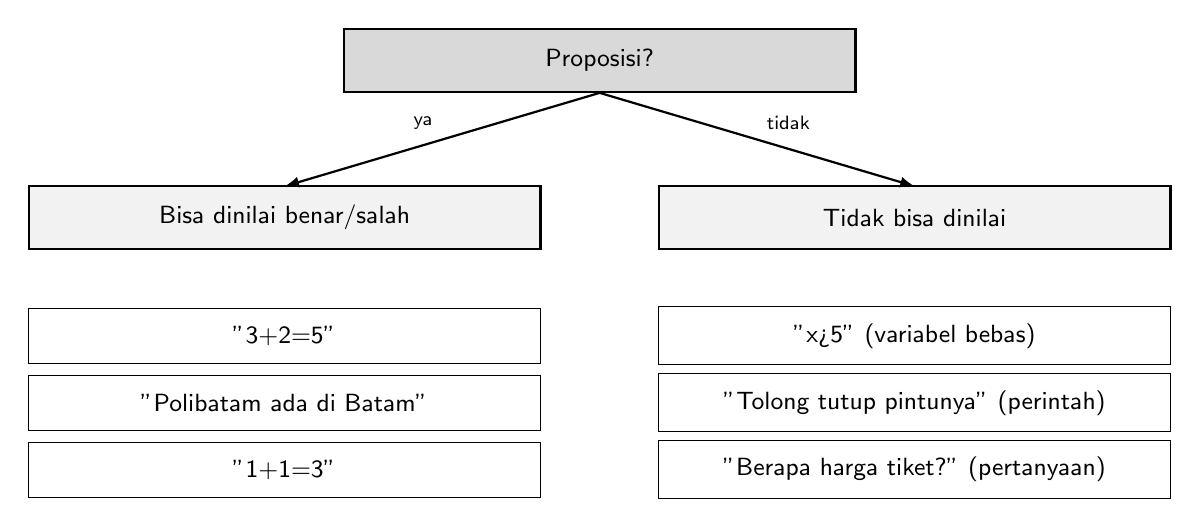
\begin{tikzpicture}[
			box/.style={rectangle, draw=black, thick, minimum width=6.5cm, minimum height=0.8cm, align=center, font=\sffamily\small},
			ex/.style={rectangle, draw=black, minimum width=6.5cm, minimum height=0.7cm, align=left, font=\sffamily\small, inner sep=6pt}
		]
		\node[box, fill=black!15] (q) at (0, 3.5) {Proposisi?};
		\node[box, fill=black!5] (y) at (-4, 1.5) {Bisa dinilai benar/salah};
		\node[box, fill=black!5] (n) at (4, 1.5) {Tidak bisa dinilai};

		\draw[thick, -latex] (q.south) -- (-4, 1.9);
		\draw[thick, -latex] (q.south) -- (4, 1.9);
		\node[font=\scriptsize\sffamily, anchor=east] at (-2, 2.7) {ya};
		\node[font=\scriptsize\sffamily, anchor=west] at (2, 2.7) {tidak};

		\node[ex, fill=white] at (-4, 0) {"3+2=5"};
		\node[ex, fill=white] at (-4, -0.85) {"Polibatam ada di Batam"};
		\node[ex, fill=white] at (-4, -1.7) {"1+1=3"};

		\node[ex, fill=white] at (4, 0) {"x>5" (variabel bebas)};
		\node[ex, fill=white] at (4, -0.85) {"Tolong tutup pintunya" (perintah)};
		\node[ex, fill=white] at (4, -1.7) {"Berapa harga tiket?" (pertanyaan)};
	\end{tikzpicture}
	\caption{Diagram alur memeriksa apakah sebuah pernyataan adalah proposisi.}
	\label{fig:proposisi}
\end{figure}

Cara membaca Gambar~\ref{fig:proposisi}: gambar ini menampilkan satu kotak di atas bertuliskan "Proposisi?" dengan dua cabang panah ke bawah. Cabang kiri menuju kotak "Bisa dinilai benar/salah", cabang kanan menuju kotak "Tidak bisa dinilai". Di bawah cabang kiri ada tiga contoh pernyataan yang memenuhi syarat: "3+2=5", "Polibatam ada di Batam", dan "1+1=3". Di bawah cabang kanan ada tiga contoh pernyataan yang tidak memenuhi syarat: "x>5" karena ada variabel bebas, "Tolong tutup pintunya" karena perintah, dan "Berapa harga tiket?" karena pertanyaan. Kotak paling atas diberi latar abu-abu gelap untuk menandakan posisi keputusan. Inti pesan gambar ini adalah memeriksa proposisi hanya butuh satu pertanyaan: apakah kalimat ini bisa diputuskan benar atau salahnya tanpa informasi tambahan.

\subsection{Cara Berpikir: Memeriksa Proposisi}

Untuk memeriksa apakah sebuah kalimat adalah proposisi, ajukan dua pertanyaan berurutan. Pertama, apakah kalimat ini kalimat berita? Jika perintah, pertanyaan, atau seruan, bukan proposisi. Kedua, apakah semua variabel di dalamnya sudah diberi nilai? Jika ada variabel bebas, bukan proposisi sampai variabel itu diberi nilai.

Jika kedua pertanyaan itu dijawab, kalimat itu adalah proposisi. Jika salah satu dilanggar, kalimat itu bukan proposisi.

\section{Lima Operator Dasar}

\subsection{Analogi Setiap Operator}

Setiap operator logika punya padanan di dunia nyata. Negasi adalah tombol lampu yang ditekan sekali untuk membalik keadaan. Konjungsi adalah dua kunci yang harus dibuka bersama untuk membuka peti. Disjungsi adalah dua pintu yang salah satunya cukup dibuka untuk masuk. Implikasi adalah janji bersyarat, misalnya "kalau kamu lulus ujian, saya beri hadiah". Biimplikasi adalah lampu yang dirangkai langsung dengan sakelarnya, sehingga menyala tepat ketika sakelar ditekan dan mati tepat ketika sakelar dilepas.

\subsection{Negasi: $\neg A$}

Negasi membalik nilai kebenaran. Jika $A$ benar, $\neg A$ salah. Jika $A$ salah, $\neg A$ benar. Tabel kebenarannya sangat pendek, hanya dua baris, ditampilkan pada Tabel~\ref{tab:negasi} \cite{rosen}.

\begin{table}[H]
	\centering
	\caption{Tabel kebenaran negasi.}
	\label{tab:negasi}
	\small
	\begin{tabular}{c c}
		\toprule
		$A$ & $\neg A$ \\
		\midrule
		B & S \\
		S & B \\
		\bottomrule
	\end{tabular}
\end{table}

Di perangkat lunak, negasi dipakai untuk membalik kondisi. Contoh: $A$ adalah "akun sedang diblokir", maka $\neg A$ adalah "akun tidak sedang diblokir". Di kode: \texttt{if (!isBlocked) \{ ... \}}. Tanda seru adalah operator negasi di hampir semua bahasa pemrograman.

\subsection{Konjungsi: $A \wedge B$}

Konjungsi bernilai benar hanya jika $A$ dan $B$ keduanya benar. Jika salah satu salah, hasilnya salah. Tabel kebenarannya ditampilkan pada Tabel~\ref{tab:konjungsi}.

\begin{table}[H]
	\centering
	\caption{Tabel kebenaran konjungsi.}
	\label{tab:konjungsi}
	\small
	\begin{tabular}{c c c}
		\toprule
		$A$ & $B$ & $A \wedge B$ \\
		\midrule
		B & B & B \\
		B & S & S \\
		S & B & S \\
		S & S & S \\
		\bottomrule
	\end{tabular}
\end{table}

Di perangkat lunak, konjungsi dipakai untuk syarat yang harus dipenuhi semua. Contoh: $L$ adalah "login valid" dan $A$ adalah "berperan sebagai admin", maka $L \wedge A$ adalah "login valid dan berperan admin". Di kode: \texttt{if (isLoggedIn \&\& isAdmin) \{ tampilkanDashboard(); \}}.

\subsection{Disjungsi: $A \vee B$}

Disjungsi bernilai benar jika salah satu dari $A$ atau $B$ benar, termasuk jika keduanya benar. Disjungsi hanya bernilai salah jika keduanya salah. Tabel kebenarannya ditampilkan pada Tabel~\ref{tab:disjungsi}.

\begin{table}[H]
	\centering
	\caption{Tabel kebenaran disjungsi.}
	\label{tab:disjungsi}
	\small
	\begin{tabular}{c c c}
		\toprule
		$A$ & $B$ & $A \vee B$ \\
		\midrule
		B & B & B \\
		B & S & B \\
		S & B & B \\
		S & S & S \\
		\bottomrule
	\end{tabular}
\end{table}

Disjungsi di tabel ini adalah disjungsi inklusif, artinya kedua-duanya boleh benar sekaligus. Ini berbeda dari disjungsi eksklusif (XOR) yang hanya benar jika tepat satu yang benar. Di perangkat lunak, disjungsi inklusif diwakili operator \texttt{||} atau \texttt{or}. Contoh: syarat diskon adalah pelanggan baru atau member premium, dan pelanggan yang baru sekaligus premium juga berhak mendapat diskon.

\subsection{Implikasi: $A \to B$}

Implikasi bernilai salah hanya jika $A$ benar tetapi $B$ salah. Semua kombinasi lain bernilai benar, termasuk kombinasi ketika $A$ salah. Tabel kebenarannya ditampilkan pada Tabel~\ref{tab:implikasi}.

\begin{table}[H]
	\centering
	\caption{Tabel kebenaran implikasi.}
	\label{tab:implikasi}
	\small
	\begin{tabular}{c c c}
		\toprule
		$A$ & $B$ & $A \to B$ \\
		\midrule
		B & B & B \\
		B & S & S \\
		S & B & B \\
		S & S & B \\
		\bottomrule
	\end{tabular}
\end{table}

Implikasi adalah operator yang paling sering membingungkan. Alasannya, implikasi tidak berbicara tentang sebab-akibat, melainkan tentang janji bersyarat. Jika saya berkata "jika hujan, maka jalan basah", janji itu dilanggar hanya jika hujan turun tetapi jalan tidak basah. Jika hujan tidak turun, janji itu tidak dilanggar, apa pun kondisi jalannya. Logika menyebut keadaan ini \textit{vacuously true}, benar karena syaratnya tidak dipenuhi. Perhatikan Gambar~\ref{fig:implikasi}.

\begin{figure}[H]
	\centering
	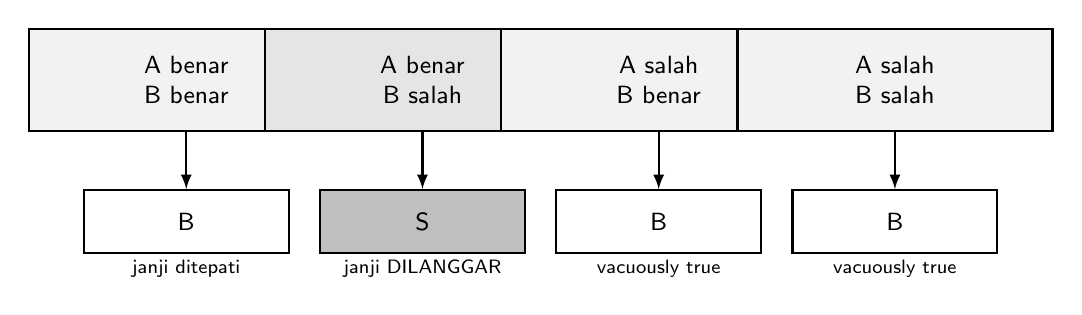
\begin{tikzpicture}[
			box/.style={rectangle, draw=black, thick, minimum width=4cm, minimum height=1.3cm, align=center, font=\sffamily\small, inner sep=6pt},
			result/.style={rectangle, draw=black, thick, minimum width=2.6cm, minimum height=0.8cm, align=center, font=\sffamily\small}
		]
		\node[box, fill=black!5] (case1) at (-4.5, 0) {A benar\\B benar};
		\node[box, fill=black!10] (case2) at (-1.5, 0) {A benar\\B salah};
		\node[box, fill=black!5] (case3) at (1.5, 0) {A salah\\B benar};
		\node[box, fill=black!5] (case4) at (4.5, 0) {A salah\\B salah};

		\node[result, fill=white] (r1) at (-4.5, -1.8) {B};
		\node[result, fill=black!25] (r2) at (-1.5, -1.8) {S};
		\node[result, fill=white] (r3) at (1.5, -1.8) {B};
		\node[result, fill=white] (r4) at (4.5, -1.8) {B};

		\draw[thick, -latex] (case1) -- (r1);
		\draw[thick, -latex] (case2) -- (r2);
		\draw[thick, -latex] (case3) -- (r3);
		\draw[thick, -latex] (case4) -- (r4);

		\node[font=\scriptsize\sffamily] at (-4.5, -2.4) {janji ditepati};
		\node[font=\scriptsize\sffamily] at (-1.5, -2.4) {janji DILANGGAR};
		\node[font=\scriptsize\sffamily] at (1.5, -2.4) {vacuously true};
		\node[font=\scriptsize\sffamily] at (4.5, -2.4) {vacuously true};
	\end{tikzpicture}
	\caption{Empat skenario implikasi $A \to B$: hanya skenario kedua yang bernilai salah.}
	\label{fig:implikasi}
\end{figure}

Cara membaca Gambar~\ref{fig:implikasi}: gambar ini menampilkan empat kotak berjajar di atas, masing-masing berisi kombinasi nilai $A$ dan $B$. Kotak pertama berisi "A benar, B benar". Kotak kedua berisi "A benar, B salah". Kotak ketiga berisi "A salah, B benar". Kotak keempat berisi "A salah, B salah". Di bawah setiap kotak ada panah yang menunjuk ke kotak hasil berisi B atau S. Hanya kotak kedua yang hasilnya S dan diberi latar abu-abu gelap. Tiga kotak lain hasilnya B. Di bawah setiap kotak hasil ada keterangan: "janji ditepati" untuk kotak pertama, "janji DILANGGAR" untuk kotak kedua, dan "vacuously true" untuk kotak ketiga dan keempat. Inti pesan gambar ini adalah implikasi hanya salah ketika syarat terpenuhi tetapi akibat tidak terjadi.

Di perangkat lunak, implikasi muncul sebagai syarat validasi. Contoh: "jika form dikirim, maka semua field wajib terisi". Ini diterjemahkan menjadi "jika bukan form dikirim, atau semua field terisi", karena $A \to B$ setara dengan $\neg A \vee B$. Kesetaraan ini dibahas pada Bagian~\ref{sec:ekivalensi}.

\subsection{Biimplikasi: $A \leftrightarrow B$}

Biimplikasi bernilai benar ketika $A$ dan $B$ bernilai sama, keduanya benar atau keduanya salah. Tabel kebenarannya ditampilkan pada Tabel~\ref{tab:biimplikasi}.

\begin{table}[H]
	\centering
	\caption{Tabel kebenaran biimplikasi.}
	\label{tab:biimplikasi}
	\small
	\begin{tabular}{c c c}
		\toprule
		$A$ & $B$ & $A \leftrightarrow B$ \\
		\midrule
		B & B & B \\
		B & S & S \\
		S & B & S \\
		S & S & B \\
		\bottomrule
	\end{tabular}
\end{table}

Di perangkat lunak, biimplikasi muncul sebagai perbandingan kesamaan. Contoh: "toggle lampu menyala jika dan hanya jika sakelar dalam posisi ON". Ekspresinya adalah \texttt{lampuMenyala == sakelarOn}. Operator perbandingan \texttt{==} pada boolean berperilaku seperti biimplikasi.

\subsection{Ringkasan Lima Operator}

Gambar~\ref{fig:lima-operator} menyandingkan kelima tabel kebenaran dalam satu pandangan.

\begin{figure}[H]
	\centering
	\resizebox{\textwidth}{!}{%
	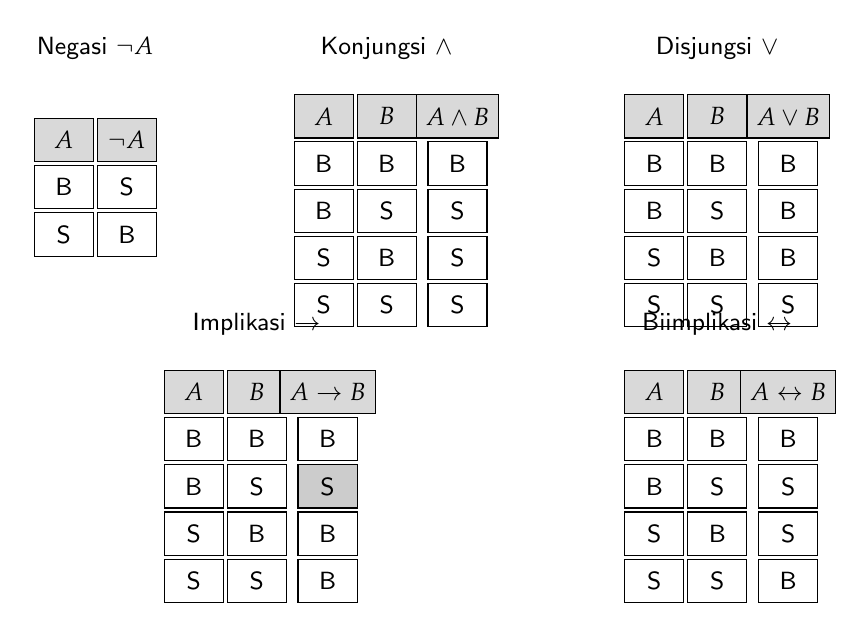
\begin{tikzpicture}[
			cell/.style={rectangle, draw=black, minimum width=0.75cm, minimum height=0.55cm, align=center, font=\small\sffamily},
			hdr/.style={cell, fill=black!15, font=\small\sffamily\bfseries}
		]
		\begin{scope}[shift={(-7.5, 0)}]
			\node[font=\sffamily\small, anchor=south] at (0.4, 1.8) {Negasi $\neg A$};
			\node[hdr] at (0, 0.9) {$A$};
			\node[hdr] at (0.8, 0.9) {$\neg A$};
			\node[cell] at (0, 0.3) {B};
			\node[cell] at (0.8, 0.3) {S};
			\node[cell] at (0, -0.3) {S};
			\node[cell] at (0.8, -0.3) {B};
		\end{scope}
		\begin{scope}[shift={(-4.2, 0)}]
			\node[font=\sffamily\small, anchor=south] at (0.8, 1.8) {Konjungsi $\wedge$};
			\node[hdr] at (0, 1.2) {$A$};
			\node[hdr] at (0.8, 1.2) {$B$};
			\node[hdr] at (1.7, 1.2) {$A \wedge B$};
			\node[cell] at (0, 0.6) {B};
			\node[cell] at (0.8, 0.6) {B};
			\node[cell] at (1.7, 0.6) {B};
			\node[cell] at (0, 0) {B};
			\node[cell] at (0.8, 0) {S};
			\node[cell] at (1.7, 0) {S};
			\node[cell] at (0, -0.6) {S};
			\node[cell] at (0.8, -0.6) {B};
			\node[cell] at (1.7, -0.6) {S};
			\node[cell] at (0, -1.2) {S};
			\node[cell] at (0.8, -1.2) {S};
			\node[cell] at (1.7, -1.2) {S};
		\end{scope}
		\begin{scope}[shift={(0, 0)}]
			\node[font=\sffamily\small, anchor=south] at (0.8, 1.8) {Disjungsi $\vee$};
			\node[hdr] at (0, 1.2) {$A$};
			\node[hdr] at (0.8, 1.2) {$B$};
			\node[hdr] at (1.7, 1.2) {$A \vee B$};
			\node[cell] at (0, 0.6) {B};
			\node[cell] at (0.8, 0.6) {B};
			\node[cell] at (1.7, 0.6) {B};
			\node[cell] at (0, 0) {B};
			\node[cell] at (0.8, 0) {S};
			\node[cell] at (1.7, 0) {B};
			\node[cell] at (0, -0.6) {S};
			\node[cell] at (0.8, -0.6) {B};
			\node[cell] at (1.7, -0.6) {B};
			\node[cell] at (0, -1.2) {S};
			\node[cell] at (0.8, -1.2) {S};
			\node[cell] at (1.7, -1.2) {S};
		\end{scope}

		\begin{scope}[shift={(-5.85, -3.5)}]
			\node[font=\sffamily\small, anchor=south] at (0.8, 1.8) {Implikasi $\to$};
			\node[hdr] at (0, 1.2) {$A$};
			\node[hdr] at (0.8, 1.2) {$B$};
			\node[hdr] at (1.7, 1.2) {$A \to B$};
			\node[cell] at (0, 0.6) {B};
			\node[cell] at (0.8, 0.6) {B};
			\node[cell] at (1.7, 0.6) {B};
			\node[cell] at (0, 0) {B};
			\node[cell] at (0.8, 0) {S};
			\node[cell, fill=black!20] at (1.7, 0) {S};
			\node[cell] at (0, -0.6) {S};
			\node[cell] at (0.8, -0.6) {B};
			\node[cell] at (1.7, -0.6) {B};
			\node[cell] at (0, -1.2) {S};
			\node[cell] at (0.8, -1.2) {S};
			\node[cell] at (1.7, -1.2) {B};
		\end{scope}
		\begin{scope}[shift={(0, -3.5)}]
			\node[font=\sffamily\small, anchor=south] at (0.8, 1.8) {Biimplikasi $\leftrightarrow$};
			\node[hdr] at (0, 1.2) {$A$};
			\node[hdr] at (0.8, 1.2) {$B$};
			\node[hdr] at (1.7, 1.2) {$A \leftrightarrow B$};
			\node[cell] at (0, 0.6) {B};
			\node[cell] at (0.8, 0.6) {B};
			\node[cell] at (1.7, 0.6) {B};
			\node[cell] at (0, 0) {B};
			\node[cell] at (0.8, 0) {S};
			\node[cell] at (1.7, 0) {S};
			\node[cell] at (0, -0.6) {S};
			\node[cell] at (0.8, -0.6) {B};
			\node[cell] at (1.7, -0.6) {S};
			\node[cell] at (0, -1.2) {S};
			\node[cell] at (0.8, -1.2) {S};
			\node[cell] at (1.7, -1.2) {B};
		\end{scope}
	\end{tikzpicture}}
	\caption{Kelima tabel kebenaran operator dasar dalam satu pandangan.}
	\label{fig:lima-operator}
\end{figure}

Cara membaca Gambar~\ref{fig:lima-operator}: gambar ini menampilkan lima tabel kecil yang tersusun dua baris. Baris atas dari kiri ke kanan berisi tabel negasi dengan dua baris data, tabel konjungsi dengan empat baris data, dan tabel disjungsi dengan empat baris data. Baris bawah berisi tabel implikasi dan tabel biimplikasi, masing-masing dengan empat baris data. Header kolom setiap tabel diberi latar abu-abu muda. Pada tabel implikasi, sel yang bernilai S di baris kedua (ketika $A$ benar tetapi $B$ salah) diberi latar abu-abu lebih gelap untuk menandakan bahwa hanya kombinasi itu yang salah. Kolom hasil setiap tabel diletakkan di kolom paling kanan. Inti pesan gambar ini adalah setiap operator punya pola kebenaran yang berbeda, dan pola itu bisa dibaca dari kolom hasil.

\subsection{Ringkasan}

Tabel~\ref{tab:lima-operator} merangkum kelima operator dengan padanan di perangkat lunak.

\begin{table}[H]
	\centering
	\caption{Ringkasan lima operator logika dan padanannya di perangkat lunak.}
	\label{tab:lima-operator}
	\small
	\begin{tabularx}{\textwidth}{l l X X}
		\toprule
		Nama & Simbol & Kapan benar & Padanan kode \\
		\midrule
		Negasi & $\neg A$ & ketika $A$ salah & \texttt{!A} \\
		Konjungsi & $A \wedge B$ & keduanya benar & \texttt{A \&\& B} \\
		Disjungsi & $A \vee B$ & salah satu atau keduanya benar & \texttt{A || B} \\
		Implikasi & $A \to B$ & kecuali $A$ benar dan $B$ salah & \texttt{!A || B} \\
		Biimplikasi & $A \leftrightarrow B$ & keduanya sama & \texttt{A == B} \\
		\bottomrule
	\end{tabularx}
\end{table}

\section{Membangun Tabel Kebenaran Majemuk}

\subsection{Analogi: Menyusun Jadwal Latihan}

Bayangkan seorang pelatih yang ingin menyusun jadwal latihan untuk tiga atlet. Setiap atlet bisa hadir atau tidak hadir, sehingga ada delapan kemungkinan kombinasi kehadiran. Untuk memastikan tidak ada kombinasi yang terlewat, pelatih menulis semua kemungkinan secara sistematis, dari yang paling banyak hadir sampai yang paling sedikit.

Tabel kebenaran dibangun dengan cara yang sama. Untuk $n$ variabel, ada $2^n$ kombinasi. Kombinasi disusun secara sistematis agar tidak ada yang terlewat dan tidak ada yang terulang.

\subsection{Aturan Dasar}

Untuk formula dengan $n$ variabel proposisi, tabel kebenaran memiliki $2^n$ baris data. Tabel juga memiliki $n+1$ kolom minimal, yaitu $n$ kolom variabel dan satu kolom hasil akhir. Jika ada sub-ekspresi di dalam formula, kolom tambahan diperlukan untuk setiap sub-ekspresi \cite{rosen}.

Ada tiga langkah menyusun tabel kebenaran. Langkah pertama, daftar semua kombinasi nilai variabel. Cara termudah adalah menganggap variabel pertama berganti setiap $2^{n-1}$ baris, variabel kedua berganti setiap $2^{n-2}$ baris, dan seterusnya. Langkah kedua, hitung sub-ekspresi dari dalam ke luar sesuai urutan operator. Langkah ketiga, isi kolom hasil akhir berdasarkan sub-ekspresi terakhir.

\subsection{Contoh: $W=(\neg A \vee B) \wedge (\neg B \vee A)$}

Formula ini memiliki dua variabel, sehingga ada $2^2=4$ baris. Sub-ekspresi yang perlu dihitung ada empat: $\neg A$, $\neg A \vee B$, $\neg B$, dan $\neg B \vee A$. Setelah itu, kolom hasil akhir dihitung dari konjungsi kedua sub-ekspresi tengah.

Baris pertama, $A=B$ dan $B=B$. $\neg A=S$, $\neg A \vee B=B$. $\neg B=S$, $\neg B \vee A=B$. Konjungsi $B \wedge B=B$.

Baris kedua, $A=B$ dan $B=S$. $\neg A=S$, $\neg A \vee B=S$. $\neg B=B$, $\neg B \vee A=B$. Konjungsi $S \wedge B=S$.

Baris ketiga, $A=S$ dan $B=B$. $\neg A=B$, $\neg A \vee B=B$. $\neg B=S$, $\neg B \vee A=S$. Konjungsi $B \wedge S=S$.

Baris keempat, $A=S$ dan $B=S$. $\neg A=B$, $\neg A \vee B=B$. $\neg B=B$, $\neg B \vee A=B$. Konjungsi $B \wedge B=B$.

Hasil akhir: B, S, S, B untuk empat baris. Perhatikan Gambar~\ref{fig:tabel-flow}.

\begin{figure}[H]
	\centering
	\begin{tikzpicture}[
			step/.style={rectangle, draw=black, thick, fill=black!5, text width=9cm, align=left, minimum height=0.7cm, font=\sffamily\small, inner sep=8pt},
			line/.style={draw, thick, -latex}
		]
		\node[step] (s1) {\textbf{Langkah 1.} Hitung $n$ variabel, tentukan $2^n$ baris};
		\node[step, below=0.25cm of s1] (s2) {\textbf{Langkah 2.} Daftar semua kombinasi secara sistematis};
		\node[step, below=0.25cm of s2] (s3) {\textbf{Langkah 3.} Hitung sub-ekspresi terdalam lebih dulu};
		\node[step, below=0.25cm of s3] (s4) {\textbf{Langkah 4.} Naik ke sub-ekspresi luar};
		\node[step, below=0.25cm of s4] (s5) {\textbf{Langkah 5.} Isi kolom hasil akhir};
		\node[step, below=0.25cm of s5] (s6) {\textbf{Langkah 6.} Klasifikasi: tautologi, kontradiksi, kontingensi};
		\draw[line] (s1) -- (s2);
		\draw[line] (s2) -- (s3);
		\draw[line] (s3) -- (s4);
		\draw[line] (s4) -- (s5);
		\draw[line] (s5) -- (s6);
	\end{tikzpicture}
	\caption{Alur enam langkah membangun tabel kebenaran majemuk.}
	\label{fig:tabel-flow}
\end{figure}

Cara membaca Gambar~\ref{fig:tabel-flow}: gambar ini menampilkan enam kotak persegi panjang tersusun dari atas ke bawah. Setiap kotak berisi satu langkah, diawali dengan angka. Kotak pertama "Hitung n variabel, tentukan 2^n baris". Kotak kedua "Daftar semua kombinasi secara sistematis". Kotak ketiga "Hitung sub-ekspresi terdalam lebih dulu". Kotak keempat "Naik ke sub-ekspresi luar". Kotak kelima "Isi kolom hasil akhir". Kotak keenam "Klasifikasi: tautologi, kontradiksi, kontingensi". Setiap kotak dihubungkan ke kotak berikutnya oleh panah pendek ke bawah. Latar kotak abu-abu sangat muda. Inti pesan gambar ini adalah penyusunan tabel kebenaran berjalan berurutan dari persiapan baris, perhitungan sub-ekspresi, sampai klasifikasi hasil.

\subsection{Cara Berpikir: Urutan Kombinasi}

Saat mengisi kolom variabel, jangan mengisi acak. Mulai dari kombinasi paling atas dengan semua variabel bernilai B, lalu turunkan satu per satu seperti menghitung biner. Variabel paling kanan berganti setiap baris, variabel kedua dari kanan berganti setiap dua baris, dan seterusnya. Dengan pola ini, $2^n$ baris terisi tanpa ada yang terlewat.

Jika langkah ini dilewati dan baris diisi acak, ada risiko satu kombinasi tertulis dua kali, sedangkan kombinasi lain tidak pernah muncul. Tabel kebenaran yang tidak lengkap tidak bisa dipakai untuk membuktikan apa pun.

\subsection{Kalau Salah: Tabel Tidak Lengkap}

Tabel kebenaran yang tidak memuat semua $2^n$ kombinasi adalah tabel yang tidak berguna. Jika aturan akses punya empat variabel, ada 16 kombinasi. Tabel dengan 12 baris hanya memeriksa 75 persen kasus. Bug yang muncul pada 4 kombinasi yang hilang akan lolos dari pengujian.

Pemrogram yang mengandalkan pengujian manual biasanya hanya menguji 2 atau 3 kombinasi yang terpikir. Tabel kebenaran memaksa semua kombinasi diperiksa, sehingga bug yang tersembunyi di kombinasi jarang ikut ditemukan \cite{oregan}.

\section{Tautologi, Kontradiksi, dan Kontingensi}

\subsection{Analogi: Tiga Jenis Janji}

Bayangkan tiga jenis janji. Janji pertama selalu ditepati, apa pun kondisinya. Janji kedua selalu dilanggar, apa pun kondisinya. Janji ketiga kadang ditepati, kadang dilanggar, tergantung situasi.

Ketiga jenis janji itu adalah tautologi, kontradiksi, dan kontingensi.

\subsection{Definisi Formal}

Tautologi adalah ekspresi logika yang selalu bernilai benar untuk semua kombinasi nilai variabelnya. Kontradiksi adalah ekspresi yang selalu bernilai salah. Kontingensi adalah ekspresi yang kadang benar, kadang salah, tergantung nilai variabelnya \cite{rosen}.

Contoh tautologi: $A \vee \neg A$. Ini disebut \textit{excluded middle}, karena setiap proposisi pasti benar atau salah, tidak ada jalan tengah.

Contoh kontradiksi: $A \wedge \neg A$. Ini disebut \textit{contradiction}, karena sebuah proposisi tidak mungkin benar sekaligus salah.

Contoh kontingensi: $A \vee B$. Hasilnya benar pada tiga kombinasi, salah pada satu kombinasi. Perhatikan Gambar~\ref{fig:tiga-jenis}.

\begin{figure}[H]
	\centering
	\resizebox{\textwidth}{!}{%
	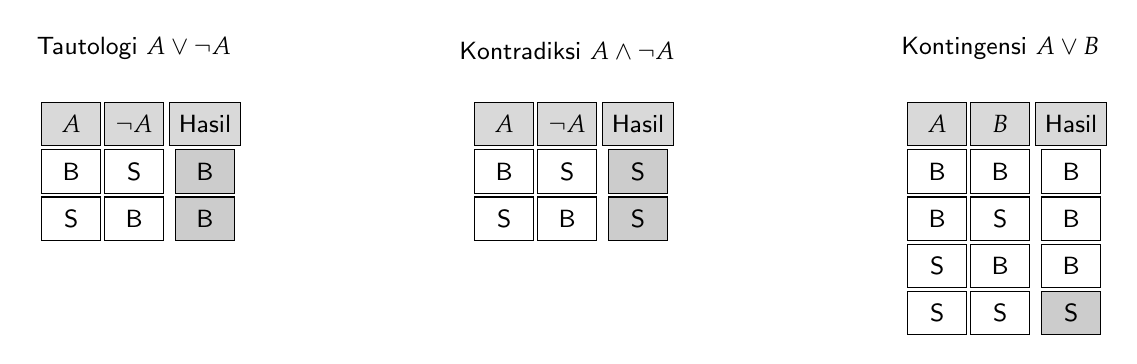
\begin{tikzpicture}[
			cell/.style={rectangle, draw=black, minimum width=0.75cm, minimum height=0.55cm, align=center, font=\small\sffamily},
			hdr/.style={cell, fill=black!15}
		]
		\begin{scope}[shift={(-5.5, 0)}]
			\node[font=\sffamily\small, anchor=south] at (0.8, 2.2) {Tautologi $A \vee \neg A$};
			\node[hdr] at (0, 1.5) {$A$};
			\node[hdr] at (0.8, 1.5) {$\neg A$};
			\node[hdr] at (1.7, 1.5) {Hasil};
			\node[cell] at (0, 0.9) {B};
			\node[cell] at (0.8, 0.9) {S};
			\node[cell, fill=black!20] at (1.7, 0.9) {B};
			\node[cell] at (0, 0.3) {S};
			\node[cell] at (0.8, 0.3) {B};
			\node[cell, fill=black!20] at (1.7, 0.3) {B};
		\end{scope}
		\begin{scope}[shift={(0, 0)}]
			\node[font=\sffamily\small, anchor=south] at (0.8, 2.2) {Kontradiksi $A \wedge \neg A$};
			\node[hdr] at (0, 1.5) {$A$};
			\node[hdr] at (0.8, 1.5) {$\neg A$};
			\node[hdr] at (1.7, 1.5) {Hasil};
			\node[cell] at (0, 0.9) {B};
			\node[cell] at (0.8, 0.9) {S};
			\node[cell, fill=black!20] at (1.7, 0.9) {S};
			\node[cell] at (0, 0.3) {S};
			\node[cell] at (0.8, 0.3) {B};
			\node[cell, fill=black!20] at (1.7, 0.3) {S};
		\end{scope}
		\begin{scope}[shift={(5.5, 0)}]
			\node[font=\sffamily\small, anchor=south] at (0.8, 2.2) {Kontingensi $A \vee B$};
			\node[hdr] at (0, 1.5) {$A$};
			\node[hdr] at (0.8, 1.5) {$B$};
			\node[hdr] at (1.7, 1.5) {Hasil};
			\node[cell] at (0, 0.9) {B};
			\node[cell] at (0.8, 0.9) {B};
			\node[cell] at (1.7, 0.9) {B};
			\node[cell] at (0, 0.3) {B};
			\node[cell] at (0.8, 0.3) {S};
			\node[cell] at (1.7, 0.3) {B};
			\node[cell] at (0, -0.3) {S};
			\node[cell] at (0.8, -0.3) {B};
			\node[cell] at (1.7, -0.3) {B};
			\node[cell] at (0, -0.9) {S};
			\node[cell] at (0.8, -0.9) {S};
			\node[cell, fill=black!20] at (1.7, -0.9) {S};
		\end{scope}
	\end{tikzpicture}}
	\caption{Tiga contoh klasifikasi ekspresi: tautologi, kontradiksi, dan kontingensi.}
	\label{fig:tiga-jenis}
\end{figure}

Cara membaca Gambar~\ref{fig:tiga-jenis}: gambar ini menampilkan tiga tabel kebenaran kecil berjajar dari kiri ke kanan. Tabel kiri berjudul "Tautologi A ∨ ¬A" dengan kolom hasil seluruhnya B dan diberi latar abu-abu. Tabel tengah berjudul "Kontradiksi A ∧ ¬A" dengan kolom hasil seluruhnya S dan diberi latar abu-abu. Tabel kanan berjudul "Kontingensi A ∨ B" dengan kolom hasil B, B, B, S, hanya satu baris yang S dan baris itu diberi latar abu-abu untuk menandakan baris pembeda. Inti pesan gambar ini adalah klasifikasi ditentukan oleh seluruh isi kolom hasil, bukan oleh satu baris saja.

\subsection{Mengapa Klasifikasi Penting}

Di perangkat lunak, tautologi adalah ekspresi yang tidak perlu ditulis karena selalu benar. Jika seorang pemrogram menulis \texttt{if (x > 0 || x <= 0)}, kondisi itu selalu benar, sehingga blok \texttt{else} tidak pernah dieksekusi. Menyadari bahwa itu tautologi membuat pemrogram menghapus kondisi yang tidak berguna.

Kontradiksi adalah ekspresi yang tidak akan pernah benar. Jika seorang pemrogram menulis \texttt{if (x > 0 \&\& x < 0)}, blok itu tidak akan pernah dieksekusi. Menyadari itu kontradiksi membuat pemrogram menyadari ada bug.

Kontingensi adalah ekspresi normal yang bergantung pada nilai. Ekspresi inilah yang biasanya dipakai.

\subsection{Cara Berpikir: Mengklasifikasi Ekspresi}

Untuk mengklasifikasi ekspresi, bangun tabel kebenaran sampai selesai, lalu periksa kolom hasil. Jika semua baris bernilai B, ekspresi itu tautologi. Jika semua baris bernilai S, ekspresi itu kontradiksi. Jika campuran, ekspresi itu kontingensi.

Jangan mengklasifikasi dari beberapa baris pertama. Satu baris yang berbeda di baris terakhir sudah cukup untuk mengubah klasifikasi dari tautologi menjadi kontingensi.

\section{Hukum-Hukum Logika}

\subsection{Analogi: Alat Tukang untuk Membongkar Ekspresi}

Bayangkan seorang tukang kayu dengan kotak perkakas berisi berbagai alat. Setiap alat punya kegunaan khusus. Palu untuk memukul, obeng untuk memutar sekrup, gergaji untuk memotong. Tukang kayu yang mengenal alatnya dapat memilih alat yang tepat tanpa harus memaksakan satu alat untuk semua pekerjaan.

Hukum-hukum logika adalah kotak perkakas itu. Setiap hukum mengubah ekspresi dengan cara yang berbeda. Pemrogram yang mengenal hukumnya dapat menyederhanakan ekspresi tanpa mengubah perilaku program.

\subsection{Sembilan Hukum Dasar}

Komutatif: $A \wedge B \equiv B \wedge A$ dan $A \vee B \equiv B \vee A$. Urutan operand tidak berpengaruh pada konjungsi dan disjungsi.

Asosiatif: $(A \wedge B) \wedge C \equiv A \wedge (B \wedge C)$ dan $(A \vee B) \vee C \equiv A \vee (B \vee C)$. Pengelompokan tiga operand tidak berpengaruh.

Distributif: $A \wedge (B \vee C) \equiv (A \wedge B) \vee (A \wedge C)$ dan $A \vee (B \wedge C) \equiv (A \vee B) \wedge (A \vee C)$. Konjungsi menyebar ke dalam disjungsi, dan sebaliknya.

Identitas: $A \wedge B \equiv A$ jika $B$ adalah Benar, dan $A \vee S \equiv A$ jika $S$ adalah Salah. Benar adalah identitas untuk konjungsi, Salah adalah identitas untuk disjungsi.

Idempoten: $A \wedge A \equiv A$ dan $A \vee A \equiv A$. Mengulang operand yang sama tidak mengubah hasil.

Dominasi: $A \vee B \equiv B$ jika $B$ adalah Benar, dan $A \wedge S \equiv S$ jika $S$ adalah Salah. Benar mendominasi disjungsi, Salah mendominasi konjungsi.

Negasi Ganda: $\neg(\neg A) \equiv A$. Membalik dua kali mengembalikan nilai asli.

Excluded Middle: $A \vee \neg A \equiv \text{Benar}$ dan $A \wedge \neg A \equiv \text{Salah}$. Sebuah proposisi pasti benar atau salah, tidak keduanya.

De Morgan: $\neg(A \wedge B) \equiv \neg A \vee \neg B$ dan $\neg(A \vee B) \equiv \neg A \wedge \neg B$. Negasi masuk ke dalam dengan membalik operator. Perhatikan Gambar~\ref{fig:de-morgan}.

\begin{figure}[H]
	\centering
	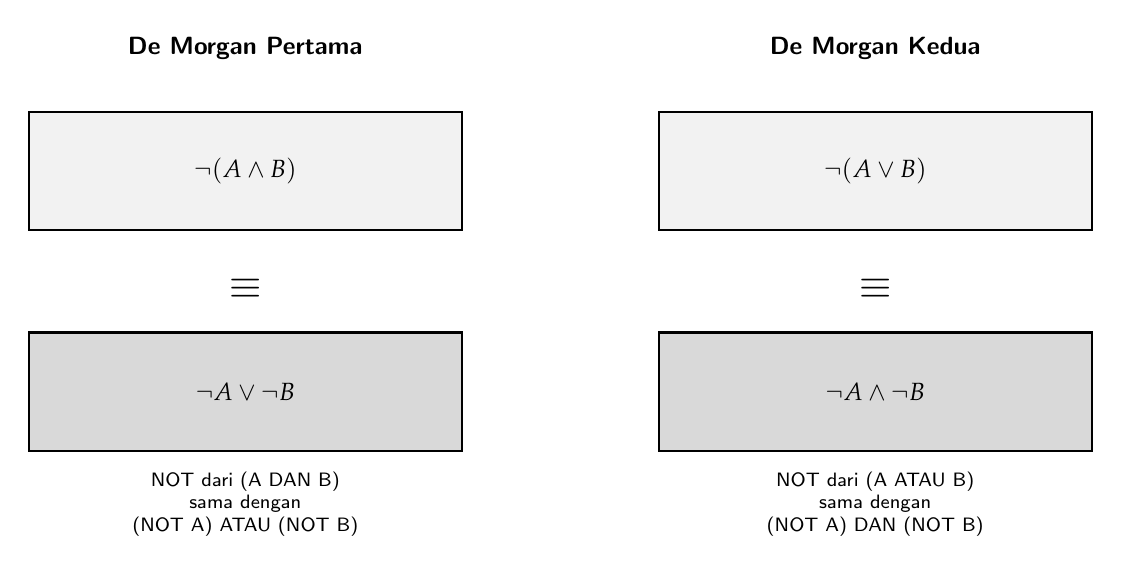
\begin{tikzpicture}[
			box/.style={rectangle, draw=black, thick, minimum width=5.5cm, minimum height=1.5cm, align=center, font=\sffamily\small, inner sep=8pt},
			hdr/.style={font=\sffamily\small\bfseries, anchor=south}
		]
		\node[hdr] at (-4, 1.8) {De Morgan Pertama};
		\node[box, fill=black!5] at (-4, 0.5) {$\neg(A \wedge B)$};
		\node[font=\Large\sffamily] at (-4, -1.0) {$\equiv$};
		\node[box, fill=black!15] at (-4, -2.3) {$\neg A \vee \neg B$};
		\node[font=\scriptsize\sffamily, anchor=north, align=center] at (-4, -3.2) {NOT dari (A DAN B)\\sama dengan\\(NOT A) ATAU (NOT B)};

		\node[hdr] at (4, 1.8) {De Morgan Kedua};
		\node[box, fill=black!5] at (4, 0.5) {$\neg(A \vee B)$};
		\node[font=\Large\sffamily] at (4, -1.0) {$\equiv$};
		\node[box, fill=black!15] at (4, -2.3) {$\neg A \wedge \neg B$};
		\node[font=\scriptsize\sffamily, anchor=north, align=center] at (4, -3.2) {NOT dari (A ATAU B)\\sama dengan\\(NOT A) DAN (NOT B)};
	\end{tikzpicture}
	\caption{Dua bentuk De Morgan: negasi masuk ke dalam dan operator dibalik.}
	\label{fig:de-morgan}
\end{figure}

Cara membaca Gambar~\ref{fig:de-morgan}: gambar ini menampilkan dua kolom berjajar. Kolom kiri berjudul "De Morgan Pertama" dengan tiga kotak bertumpuk. Kotak atas berisi $\neg(A \wedge B)$, kotak tengah berisi tanda $\equiv$, kotak bawah berisi $\neg A \vee \neg B$. Di bawahnya ada keterangan "NOT dari (A DAN B) sama dengan (NOT A) ATAU (NOT B)". Kolom kanan berjudul "De Morgan Kedua" dengan pola serupa: $\neg(A \vee B)$ di atas, tanda $\equiv$ di tengah, $\neg A \wedge \neg B$ di bawah, dan keterangan "NOT dari (A ATAU B) sama dengan (NOT A) DAN (NOT B)". Kotak bawah kedua kolom diberi latar abu-abu lebih gelap untuk menandakan bentuk hasil. Inti pesan gambar ini adalah De Morgan menukar peran DAN dan ATAU sambil memindahkan negasi ke setiap operand.

\subsection{Ringkasan}

Tabel~\ref{tab:hukum} merangkum sembilan hukum logika.

\begin{table}[H]
	\centering
	\caption{Ringkasan hukum-hukum logika proposisi.}
	\label{tab:hukum}
	\small
	\begin{tabularx}{\textwidth}{l X}
		\toprule
		Nama hukum & Bentuk \\
		\midrule
		Komutatif & $A \wedge B \equiv B \wedge A$; $A \vee B \equiv B \vee A$ \\
		Asosiatif & $(A \wedge B) \wedge C \equiv A \wedge (B \wedge C)$ \\
		Distributif & $A \wedge (B \vee C) \equiv (A \wedge B) \vee (A \wedge C)$ \\
		Identitas & $A \wedge \text{Benar} \equiv A$; $A \vee \text{Salah} \equiv A$ \\
		Idempoten & $A \wedge A \equiv A$; $A \vee A \equiv A$ \\
		Dominasi & $A \vee \text{Benar} \equiv \text{Benar}$; $A \wedge \text{Salah} \equiv \text{Salah}$ \\
		Negasi Ganda & $\neg(\neg A) \equiv A$ \\
		Excluded Middle & $A \vee \neg A \equiv \text{Benar}$; $A \wedge \neg A \equiv \text{Salah}$ \\
		De Morgan & $\neg(A \wedge B) \equiv \neg A \vee \neg B$; $\neg(A \vee B) \equiv \neg A \wedge \neg B$ \\
		\bottomrule
	\end{tabularx}
\end{table}

\subsection{Mengapa Hukum Logika Penting}

Hukum logika dipakai untuk menyederhanakan ekspresi tanpa harus membangun tabel kebenaran. Jika ekspresi awal punya 4 variabel, tabel kebenarannya 16 baris. Jika ekspresi bisa disederhanakan menjadi 2 variabel, tabel kebenarannya hanya 4 baris. Pengujian menjadi lebih cepat dan lebih mudah dibaca.

Selain itu, hukum logika dipakai untuk membuktikan bahwa dua ekspresi ekivalen. Bukti dengan tabel kebenaran memerlukan 16 baris, sedangkan bukti dengan hukum logika hanya memerlukan beberapa langkah.

\section{Ekivalensi Logis dan De Morgan}
\label{sec:ekivalensi}

\subsection{Analogi: Dua Resep yang Hasilnya Sama}

Bayangkan dua resep kue. Resep pertama memakai mentega dan gula. Resep kedua memakai gula dan mentega. Kedua resep itu berbeda urutan bahannya, tetapi menghasilkan kue yang sama.

Dua ekspresi logika disebut ekivalen jika keduanya selalu bernilai sama untuk setiap kombinasi nilai variabelnya. Notasinya $W_1 \equiv W_2$.

\subsection{Cara Membuktikan Ekivalensi}

Ada dua cara membuktikan ekivalensi. Cara pertama dengan tabel kebenaran: bangun tabel untuk kedua ekspresi, lalu bandingkan kolom hasilnya. Jika setiap baris bernilai sama, kedua ekspresi ekivalen. Cara kedua dengan hukum logika: ubah ekspresi pertama langkah demi langkah sampai bentuknya sama dengan ekspresi kedua.

Contoh klasik: buktikan $A \to B \equiv \neg A \vee B$. Bukti dengan tabel kebenaran ditampilkan pada Tabel~\ref{tab:ekivalensi-implikasi}.

\begin{table}[H]
	\centering
	\caption{Bukti ekivalensi $A \to B \equiv \neg A \vee B$ dengan tabel kebenaran.}
	\label{tab:ekivalensi-implikasi}
	\small
	\begin{tabular}{c c c c c}
		\toprule
		$A$ & $B$ & $A \to B$ & $\neg A$ & $\neg A \vee B$ \\
		\midrule
		B & B & B & S & B \\
		B & S & S & S & S \\
		S & B & B & B & B \\
		S & S & B & B & B \\
		\bottomrule
	\end{tabular}
\end{table}

Kolom ketiga dan kolom kelima identik di setiap baris, sehingga kedua ekspresi ekivalen. Ekivalensi ini dipakai di perangkat lunak untuk menuliskan implikasi dalam bentuk yang lebih mudah dievaluasi oleh komputer.

\subsection{De Morgan di Perangkat Lunak}

De Morgan sering muncul saat menyederhanakan kondisi negasi. Contoh: \texttt{!(isLoggedIn \&\& isAdmin)} setara dengan \texttt{!isLoggedIn || !isAdmin}. Keduanya bernilai benar ketika pengguna bukan admin atau belum login.

De Morgan juga dipakai untuk mengubah kondisi menjadi bentuk yang lebih mudah dibaca. Contoh: "pengguna tidak berhak mengakses" bisa ditulis sebagai $\neg(L \wedge A)$ atau sebagai $\neg L \vee \neg A$. Kedua bentuk itu sama secara logika, tetapi bentuk kedua lebih jelas menjelaskan dua alasan penolakan: belum login, atau bukan admin.

\subsection{Cara Berpikir: Memilih Cara Bukti}

Jika ekspresi hanya punya 2 variabel, tabel kebenaran dengan 4 baris lebih cepat. Jika ekspresi punya 3 variabel, tabel dengan 8 baris masih wajar. Jika ekspresi punya 4 variabel atau lebih, tabel dengan 16 baris atau lebih mulai melelahkan. Pada kasus itu, bukti dengan hukum logika lebih efisien, walaupun memerlukan pemahaman hukum.

\section{Menyederhanakan Ekspresi}

\subsection{Analogi: Membongkar Kabel yang Kusut}

Bayangkan sebuah kotak kabel yang kusut. Ada empat kabel yang saling melilit. Setelah diurai dengan teliti, ternyata keempat kabel itu hanyalah satu kabel yang dilipat empat kali. Kotak yang tampak rumit ternyata hanya berisi satu kabel sederhana.

Penyederhanaan ekspresi logika bekerja seperti mengurai kabel itu. Ekspresi yang tampak rumit diurai dengan hukum logika, dan ternyata hanya setara dengan satu kondisi sederhana.

\subsection{Contoh Lengkap}

Sederhanakan $\neg(\neg A \vee B) \vee (A \wedge B)$. Setiap langkah dijelaskan dengan nama hukum yang dipakai.

Ekspresi awal: $\neg(\neg A \vee B) \vee (A \wedge B)$.

Langkah 1, De Morgan pada $\neg(\neg A \vee B)$: $\neg(\neg A \vee B) \equiv \neg(\neg A) \wedge \neg B$. Bentuk sekarang: $(\neg(\neg A) \wedge \neg B) \vee (A \wedge B)$.

Langkah 2, Negasi Ganda pada $\neg(\neg A)$: $\neg(\neg A) \equiv A$. Bentuk sekarang: $(A \wedge \neg B) \vee (A \wedge B)$.

Langkah 3, Distributif: $A \wedge \neg B$ dan $A \wedge B$ punya faktor sama $A$, sehingga bisa difaktorkan menjadi $A \wedge (\neg B \vee B)$.

Langkah 4, Excluded Middle pada $\neg B \vee B$: $\neg B \vee B \equiv \text{Benar}$. Bentuk sekarang: $A \wedge \text{Benar}$.

Langkah 5, Identitas pada $A \wedge \text{Benar}$: $A \wedge \text{Benar} \equiv A$.

Hasil akhir: $A$. Ekspresi yang tampak rumit dengan tiga operator ternyata hanya setara dengan satu variabel. Perhatikan Gambar~\ref{fig:penyederhanaan}.

\begin{figure}[H]
	\centering
	\begin{tikzpicture}[
			step/.style={rectangle, draw=black, thick, fill=black!5, text width=10cm, align=left, minimum height=0.7cm, font=\sffamily\small, inner sep=8pt},
			lbl/.style={font=\scriptsize\sffamily, anchor=west},
			line/.style={draw, thick, -latex}
		]
		\node[step] (s1) {$\neg(\neg A \vee B) \vee (A \wedge B)$};
		\node[step, below=0.3cm of s1] (s2) {$(\neg(\neg A) \wedge \neg B) \vee (A \wedge B)$};
		\node[step, below=0.3cm of s2] (s3) {$(A \wedge \neg B) \vee (A \wedge B)$};
		\node[step, below=0.3cm of s3] (s4) {$A \wedge (\neg B \vee B)$};
		\node[step, below=0.3cm of s4] (s5) {$A \wedge \text{Benar}$};
		\node[step, fill=black!15, below=0.3cm of s5] (s6) {$A$};

		\draw[line] (s1) -- (s2);
		\draw[line] (s2) -- (s3);
		\draw[line] (s3) -- (s4);
		\draw[line] (s4) -- (s5);
		\draw[line] (s5) -- (s6);

		\node[lbl] at (5.5, -0.5) {awal};
		\node[lbl] at (5.5, -1.6) {De Morgan};
		\node[lbl] at (5.5, -2.7) {Negasi Ganda};
		\node[lbl] at (5.5, -3.8) {Distributif};
		\node[lbl] at (5.5, -4.9) {Excluded Middle};
		\node[lbl] at (5.5, -6.0) {Identitas};
	\end{tikzpicture}
	\caption{Alur penyederhanaan ekspresi dengan nama hukum di setiap langkah.}
	\label{fig:penyederhanaan}
\end{figure}

Cara membaca Gambar~\ref{fig:penyederhanaan}: gambar ini menampilkan enam kotak persegi panjang tersusun dari atas ke bawah. Setiap kotak berisi satu bentuk ekspresi. Kotak pertama ekspresi awal $\neg(\neg A \vee B) \vee (A \wedge B)$. Kotak kedua hasil De Morgan. Kotak ketiga hasil Negasi Ganda. Kotak keempat hasil Distributif. Kotak kelima hasil Excluded Middle. Kotak keenam hasil Identitas, yaitu $A$, dengan latar abu-abu lebih gelap untuk menandakan hasil akhir. Di sebelah kanan setiap kotak ada label nama hukum yang dipakai. Panah menghubungkan kotak dari atas ke bawah. Inti pesan gambar ini adalah setiap langkah penyederhanaan dijelaskan oleh satu nama hukum, dan hasil akhirnya jauh lebih sederhana dari ekspresi awal.

\subsection{Mengapa Penyederhanaan Penting}

Kode warisan (legacy code) sering berisi kondisi boolean yang berlebihan. Ekspresi yang sama ditulis berkali-kali dengan bentuk berbeda. Penyederhanaan dengan hukum logika membuat kode lebih pendek, lebih mudah dibaca, dan lebih mudah diuji, tanpa mengubah perilaku program.

Selain itu, penyederhanaan mengurangi jumlah kasus uji. Ekspresi dengan 4 variabel memerlukan 16 kasus uji. Ekspresi yang sudah disederhanakan menjadi 1 variabel hanya memerlukan 2 kasus uji. Penghematan waktu pengujian ini sangat berarti pada sistem besar \cite{sommerville}.

\subsection{Kalau Salah: Menyederhanakan dengan Menghapus Operator}

Kesalahan paling sering adalah menyederhanakan dengan menghapus operator yang tampak tidak perlu. Contoh: mengira $\neg(A \wedge B)$ sama dengan $\neg A \wedge \neg B$. Bentuk kedua itu salah, karena De Morgan mengubah $\wedge$ menjadi $\vee$.

Perbedaan ini bukan sepele. Jika $A=B$ dan $B=S$, maka $\neg(A \wedge B)=\neg(B \wedge S)=\neg S=B$, sedangkan $\neg A \wedge \neg B=S \wedge B=S$. Kedua hasil berbeda. Kode yang memakai bentuk salah akan menolak pengguna yang seharusnya diterima, atau menerima pengguna yang seharusnya ditolak.

\section{Studi Kasus 1: Validasi Akses Dashboard Admin}

\subsection{Langkah 1: Definisikan Proposisi}

Sistem Informasi Akademik memiliki halaman dashboard admin yang hanya boleh dibuka oleh pengguna tertentu. Ada empat proposisi yang terlibat. $L$ berarti "login pengguna valid". $A$ berarti "pengguna berperan sebagai admin". $O$ berarti "kode OTP tervalidasi". $B$ berarti "akun sedang diblokir".

Keempat proposisi itu bukan variabel bebas. Setiap pengguna punya nilai pasti untuk keempatnya. Login bisa valid atau tidak valid. Peran bisa admin atau bukan admin. OTP bisa tervalidasi atau tidak. Akun bisa diblokir atau tidak.

\subsection{Langkah 2: Rumuskan Aturan}

Aturan dalam bahasa natural: "Akses diizinkan jika pengguna login valid, berperan admin, OTP tervalidasi, dan akun tidak sedang diblokir."

Aturan ini punya empat syarat yang harus dipenuhi semua. Kata "dan" menandakan konjungsi. Syarat keempat adalah "tidak sedang diblokir", yang merupakan negasi dari $B$.

\subsection{Langkah 3: Terjemahkan ke Ekspresi Logika}

Ekspresi logikanya adalah $\text{Akses}=(L \wedge A \wedge O) \wedge \neg B$. Tanda kurung mengelompokkan tiga syarat pertama, lalu hasilnya dikonjungsi dengan negasi syarat keempat. Perhatikan Gambar~\ref{fig:dashboard-gate}.

\begin{figure}[H]
	\centering
	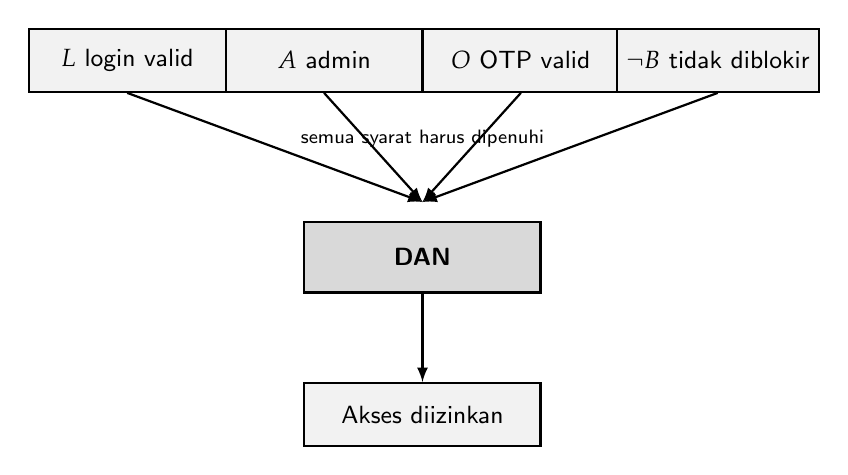
\begin{tikzpicture}[
			cond/.style={rectangle, draw=black, thick, minimum width=2.5cm, minimum height=0.8cm, align=center, font=\sffamily\small},
			gate/.style={rectangle, draw=black, thick, fill=black!15, minimum width=3cm, minimum height=0.9cm, align=center, font=\sffamily\small\bfseries},
			result/.style={rectangle, draw=black, thick, fill=black!5, minimum width=3cm, minimum height=0.8cm, align=center, font=\sffamily\small}
		]
		\node[cond, fill=black!5] (L) at (-4, 3) {$L$ login valid};
		\node[cond, fill=black!5] (A) at (-1.5, 3) {$A$ admin};
		\node[cond, fill=black!5] (O) at (1, 3) {$O$ OTP valid};
		\node[cond, fill=black!5] (B) at (3.5, 3) {$\neg B$ tidak diblokir};

		\node[gate] (gate) at (-0.25, 0.5) {DAN};
		\node[result] (res) at (-0.25, -1.5) {Akses diizinkan};

		\draw[thick, -latex] (L.south) -- (-0.25, 1.2);
		\draw[thick, -latex] (A.south) -- (-0.25, 1.2);
		\draw[thick, -latex] (O.south) -- (-0.25, 1.2);
		\draw[thick, -latex] (B.south) -- (-0.25, 1.2);
		\draw[thick, -latex] (gate.south) -- (res.north);

		\node[font=\scriptsize\sffamily, align=center] at (-0.25, 2.0) {semua syarat harus dipenuhi};
	\end{tikzpicture}
	\caption{Gerbang logika untuk aturan akses dashboard admin.}
	\label{fig:dashboard-gate}
\end{figure}

Cara membaca Gambar~\ref{fig:dashboard-gate}: gambar ini menampilkan empat kotak kondisi di bagian atas, berjajar dari kiri ke kanan: $L$ login valid, $A$ admin, $O$ OTP valid, dan $\neg B$ tidak diblokir. Keempat panah dari kotak kondisi menuju ke satu kotak tengah bertuliskan "DAN" dengan latar abu-abu gelap. Di bawah kotak "DAN" ada panah menuju kotak bawah bertuliskan "Akses diizinkan". Di atas kotak "DAN" ada keterangan "semua syarat harus dipenuhi". Inti pesan gambar ini adalah aturan akses adalah gerbang DAN dengan empat masukan, dan pintu terbuka hanya jika keempatnya bernilai benar.

\subsection{Langkah 4: Susun Tabel Kebenaran 16 Baris}

Ada empat variabel, sehingga ada $2^4=16$ baris. Tabel lengkapnya ditampilkan pada Tabel~\ref{tab:dashboard-16}.

\begin{table}[H]
	\centering
	\caption{Tabel kebenaran lengkap validasi akses dashboard admin.}
	\label{tab:dashboard-16}
	\footnotesize
	\begin{tabular}{c c c c c l}
		\toprule
		\# & $L$ & $A$ & $O$ & $B$ & Akses \\
		\midrule
		1 & B & B & B & B & S \\
		2 & B & B & B & S & B \\
		3 & B & B & S & B & S \\
		4 & B & B & S & S & S \\
		5 & B & S & B & B & S \\
		6 & B & S & B & S & S \\
		7 & B & S & S & B & S \\
		8 & B & S & S & S & S \\
		9 & S & B & B & B & S \\
		10 & S & B & B & S & S \\
		11 & S & B & S & B & S \\
		12 & S & B & S & S & S \\
		13 & S & S & B & B & S \\
		14 & S & S & B & S & S \\
		15 & S & S & S & B & S \\
		16 & S & S & S & S & S \\
		\bottomrule
	\end{tabular}
\end{table}

\subsection{Langkah 5: Identifikasi Baris yang Diizinkan}

Dari enam belas baris, hanya baris kedua yang bernilai B pada kolom Akses. Baris kedua adalah kombinasi $L=B$, $A=B$, $O=B$, dan $B=S$. Artinya, pengguna diizinkan masuk hanya ketika login valid, berperan admin, OTP tervalidasi, dan akun tidak diblokir. Semua kombinasi lain menolak akses.

Baris pertama menarik untuk diperhatikan. Pada baris pertama, semua syarat positif terpenuhi, yaitu $L=B$, $A=B$, dan $O=B$. Namun $B=B$ juga, artinya akun sedang diblokir. Akses pada baris pertama tetap S. Ini menunjukkan bahwa akun yang diblokir tetap ditolak, walaupun semua syarat lain terpenuhi. Tanpa tanda negasi pada $B$, baris pertama akan bernilai B, dan akun yang diblokir bisa masuk.

\subsection{Langkah 6: Tulis Kode Program}

Kode program yang mengimplementasikan aturan ini ditulis dengan operator yang sesuai. Konjungsi menjadi \texttt{\&\&}, negasi menjadi \texttt{!}.

\begin{lstlisting}[style=code]
if (isLoggedIn && isAdmin && otpValid && !isBlocked) {
    showAdminDashboard();
}
\end{lstlisting}

Kode itu persis mengikuti ekspresi $(L \wedge A \wedge O) \wedge \neg B$. Tidak ada operator yang ditambah, tidak ada yang dihilangkan.

\subsection{Langkah 7: Verifikasi dengan Negasi}

Cara lain memeriksa kebenaran aturan adalah memeriksa negasinya. Pengguna yang ditolak adalah negasi dari aturan akses, yaitu $\neg((L \wedge A \wedge O) \wedge \neg B)$. Dengan De Morgan, ekspresi itu menjadi $\neg L \vee \neg A \vee \neg O \vee B$. Artinya, pengguna ditolak jika tidak login, atau bukan admin, atau OTP tidak valid, atau akun diblokir.

Kedua bentuk itu ekivalen. Jika pemrogram menulis aturan penolakan, ia bisa memakai bentuk negasi. Jika ia menulis aturan penerimaan, ia bisa memakai bentuk asli. Keduanya memberi hasil yang sama.

\subsection{Langkah 8: Kesimpulan Kasus}

Aturan akses dashboard admin adalah konjungsi dari empat syarat, dengan satu syarat dinegasikan. Tabel kebenaran membuktikan aturan itu hanya mengizinkan satu dari enam belas kombinasi, dan kombinasi yang diizinkan adalah kombinasi yang masuk akal. Tanpa tabel kebenaran, pemrogram hanya akan menguji beberapa kombinasi, dan kemungkinan besar melewatkan kombinasi yang diblokir tetapi semua syarat lain terpenuhi. Alur lengkap kasus ditunjukkan pada Gambar~\ref{fig:alur-dashboard}.

\begin{figure}[H]
	\centering
	\begin{tikzpicture}[
			step/.style={rectangle, draw=black, thick, fill=black!5, text width=9cm, align=left, minimum height=0.7cm, font=\sffamily\small, inner sep=8pt},
			line/.style={draw, thick, -latex}
		]
		\node[step] (s1) {\textbf{1.} Definisikan $L$, $A$, $O$, $B$};
		\node[step, below=0.25cm of s1] (s2) {\textbf{2.} Rumuskan aturan dalam bahasa natural};
		\node[step, below=0.25cm of s2] (s3) {\textbf{3.} Terjemahkan ke ekspresi $(L \wedge A \wedge O) \wedge \neg B$};
		\node[step, below=0.25cm of s3] (s4) {\textbf{4.} Susun tabel kebenaran 16 baris};
		\node[step, below=0.25cm of s4] (s5) {\textbf{5.} Identifikasi baris yang diizinkan};
		\node[step, below=0.25cm of s5] (s6) {\textbf{6.} Tulis kode program};
		\node[step, below=0.25cm of s6] (s7) {\textbf{7.} Verifikasi dengan negasi};
		\node[step, below=0.25cm of s7] (s8) {\textbf{8.} Simpulkan};
		\draw[line] (s1) -- (s2);
		\draw[line] (s2) -- (s3);
		\draw[line] (s3) -- (s4);
		\draw[line] (s4) -- (s5);
		\draw[line] (s5) -- (s6);
		\draw[line] (s6) -- (s7);
		\draw[line] (s7) -- (s8);
	\end{tikzpicture}
	\caption{Alur delapan langkah studi kasus validasi akses dashboard admin.}
	\label{fig:alur-dashboard}
\end{figure}

Cara membaca Gambar~\ref{fig:alur-dashboard}: gambar ini menampilkan delapan kotak persegi panjang tersusun dari atas ke bawah. Setiap kotak berisi satu langkah, diawali angka tebal. Kotak pertama "Definisikan L, A, O, B". Kotak kedua "Rumuskan aturan dalam bahasa natural". Kotak ketiga "Terjemahkan ke ekspresi (L ∧ A ∧ O) ∧ ¬B". Kotak keempat "Susun tabel kebenaran 16 baris". Kotak kelima "Identifikasi baris yang diizinkan". Kotak keenam "Tulis kode program". Kotak ketujuh "Verifikasi dengan negasi". Kotak kedelapan "Simpulkan". Panah pendek ke bawah menghubungkan setiap kotak ke kotak berikutnya. Latar kotak abu-abu sangat muda. Inti pesan gambar ini adalah perancangan aturan akses berjalan berurutan dari definisi proposisi sampai verifikasi.

\section{Studi Kasus 2: Validasi Peminjaman Buku}

\subsection{Konteks}

Perpustakaan digital memiliki formulir peminjaman buku. Peminjaman diizinkan jika empat syarat terpenuhi. $K$ berarti "kartu anggota aktif". $T$ berarti "tidak ada tunggakan denda". $S$ berarti "buku berstatus tersedia". $M$ berarti "jumlah pinjaman belum melebihi batas maksimum".

\subsection{Rumusan Ekspresi}

Aturan peminjaman adalah konjungsi keempat syarat: $\text{Pinjam}=K \wedge T \wedge S \wedge M$. Tidak ada syarat yang dinegasikan, karena keempatnya dinyatakan dalam bentuk positif.

\subsection{Tabel Kebenaran 16 Baris}

Dengan empat variabel, ada 16 baris. Hasilnya ditampilkan pada Tabel~\ref{tab:peminjaman-16}.

\begin{table}[H]
	\centering
	\caption{Tabel kebenaran validasi peminjaman buku.}
	\label{tab:peminjaman-16}
	\footnotesize
	\begin{tabular}{c c c c c l}
		\toprule
		\# & $K$ & $T$ & $S$ & $M$ & Pinjam \\
		\midrule
		1 & B & B & B & B & B \\
		2 & B & B & B & S & S \\
		3 & B & B & S & B & S \\
		4 & B & B & S & S & S \\
		5 & B & S & B & B & S \\
		6 & B & S & B & S & S \\
		7 & B & S & S & B & S \\
		8 & B & S & S & S & S \\
		9 & S & B & B & B & S \\
		10 & S & B & B & S & S \\
		11 & S & B & S & B & S \\
		12 & S & B & S & S & S \\
		13 & S & S & B & B & S \\
		14 & S & S & B & S & S \\
		15 & S & S & S & B & S \\
		16 & S & S & S & S & S \\
		\bottomrule
	\end{tabular}
\end{table}

Hanya baris pertama bernilai B. Artinya, peminjaman diizinkan hanya ketika keempat syarat terpenuhi. Bandingkan dengan studi kasus sebelumnya: pada dashboard admin, hanya baris kedua yang diizinkan karena ada negasi pada $B$. Pada peminjaman buku, semua syarat dinyatakan positif, sehingga baris pertama yang diizinkan.

\subsection{Klasifikasi Ekspresi}

Ekspresi $K \wedge T \wedge S \wedge M$ adalah kontingensi. Kolom hasilnya berisi satu B dan lima belas S. Ekspresi ini tidak selalu benar, tidak selalu salah, tetapi bergantung pada nilai keempat variabel.

Ekspresi ini juga bukan tautologi, karena ada baris yang hasilnya S. Bukan kontradiksi, karena ada baris yang hasilnya B.

\subsection{Penyederhanaan}

Ekspresi $K \wedge T \wedge S \wedge M$ sudah dalam bentuk paling sederhana. Tidak ada hukum logika yang bisa mengurangi jumlah variabel, karena keempat variabel muncul satu kali dan tidak ada pasangan yang saling meniadakan. Setiap variabel berperan independen dalam menentukan hasil.

Jika pemrogram mencoba menyederhanakan dengan menghapus salah satu variabel, perilaku program berubah. Tanpa variabel $K$, mahasiswa yang kartunya tidak aktif tetap bisa meminjam. Itu tidak sesuai aturan perpustakaan.

\subsection{Mengapa Kasus Kedua Penting}

Studi kasus kedua menunjukkan bahwa tidak semua ekspresi bisa disederhanakan. Ada ekspresi yang sudah minimal, dan menyederhanakannya lebih lanjut akan mengubah perilaku. Pemrogram yang terobsesi menyederhanakan tanpa memeriksa tabel kebenaran bisa menghapus syarat yang penting.

Kedua studi kasus membentuk pasangan yang berguna. Yang pertama memiliki negasi, sehingga tabel kebenaran menunjukkan baris kedua yang diizinkan. Yang kedua tidak memiliki negasi, sehingga tabel kebenaran menunjukkan baris pertama yang diizinkan. Keduanya menyampaikan pesan yang sama: tabel kebenaran memaksa pemrogram memeriksa semua kombinasi, bukan hanya kombinasi yang terpikir.

\section{Kesalahan Umum dan Cara Menghindarinya}

Tabel~\ref{tab:kesalahan} memuat kesalahan yang paling sering muncul saat bekerja dengan logika proposisi.

\begin{table}[H]
	\centering
	\caption{Kesalahan umum pada penerapan logika proposisi.}
	\label{tab:kesalahan}
	\footnotesize
	\begin{tabularx}{\textwidth}{l X X}
		\toprule
		Kesalahan & Akibat & Perbaikan \\
		\midrule
		menganggap pertanyaan atau perintah sebagai proposisi & ekspresi tidak bisa dinilai & pastikan kalimat berita dan variabel sudah diberi nilai \\
		menulis $\wedge$ padahal maksudnya $\vee$ & aturan terlalu ketat & tentukan apakah semua atau salah satu \\
		menulis $\vee$ padahal maksudnya $\wedge$ & aturan terlalu longgar & tentukan apakah semua atau salah satu \\
		menganggap $\vee$ sebagai XOR & aturan menolak pelanggan yang memenuhi dua syarat & disjungsi inklusif, bukan eksklusif \\
		menafsirkan implikasi sebagai sebab-akibat & bingung saat $A$ salah & implikasi hanya janji bersyarat \\
		lupa negasi pada syarat blokir & akun diblokir tetap bisa masuk & periksa setiap syarat negatif \\
		De Morgan salah operator & hasil kebalikan & $\wedge$ menjadi $\vee$, $\vee$ menjadi $\wedge$ \\
		menyederhanakan tanpa cek tabel & perilaku program berubah & verifikasi dengan tabel kebenaran \\
		menguji hanya kasus normal & bug di kombinasi jarang lolos & bangun tabel kebenaran lengkap \\
		kurang tanda kurung di kode & presedensi operator salah & pakai kurung eksplisit \\
		\bottomrule
	\end{tabularx}
\end{table}

Dua kesalahan yang paling sering adalah melupakan negasi pada syarat blokir, dan menulis kode tanpa tanda kurung eksplisit. Kesalahan pertama membuat akun yang diblokir bisa masuk. Kesalahan kedua membuat \texttt{a || b \&\& c} dievaluasi sebagai \texttt{a || (b \&\& c)} padahal maksudnya \texttt{(a || b) \&\& c}. Tanda kurung eksplisit mencegah kebingungan yang berasal dari presedensi operator.

\section{Lembar Rujukan Cepat}

Tabel~\ref{tab:rujukan-cepat} adalah lembar rujukan untuk ujian atau kerja.

\begin{table}[H]
	\centering
	\caption{Lembar rujukan cepat logika proposisi.}
	\label{tab:rujukan-cepat}
	\footnotesize
	\begin{tabularx}{\textwidth}{l X}
		\toprule
		Kebutuhan & Notasi atau aturan \\
		\midrule
		proposisi & kalimat berita bernilai B atau S \\
		negasi & $\neg A$, benar jika $A$ salah \\
		konjungsi & $A \wedge B$, benar jika keduanya benar \\
		disjungsi & $A \vee B$, benar jika salah satu benar \\
		implikasi & $A \to B$, salah hanya jika $A$ benar dan $B$ salah \\
		biimplikasi & $A \leftrightarrow B$, benar jika keduanya sama \\
		jumlah baris tabel & $2^n$ untuk $n$ variabel \\
		komutatif & $A \wedge B \equiv B \wedge A$ \\
		asosiatif & $(A \wedge B) \wedge C \equiv A \wedge (B \wedge C)$ \\
		distributif & $A \wedge (B \vee C) \equiv (A \wedge B) \vee (A \wedge C)$ \\
		identitas & $A \wedge \text{B} \equiv A$; $A \vee \text{S} \equiv A$ \\
		idempoten & $A \wedge A \equiv A$ \\
		dominasi & $A \vee \text{B} \equiv \text{B}$; $A \wedge \text{S} \equiv \text{S}$ \\
		negasi ganda & $\neg(\neg A) \equiv A$ \\
		excluded middle & $A \vee \neg A \equiv \text{B}$; $A \wedge \neg A \equiv \text{S}$ \\
		De Morgan pertama & $\neg(A \wedge B) \equiv \neg A \vee \neg B$ \\
		De Morgan kedua & $\neg(A \vee B) \equiv \neg A \wedge \neg B$ \\
		ekivalensi implikasi & $A \to B \equiv \neg A \vee B$ \\
		tautologi & semua baris B \\
		kontradiksi & semua baris S \\
		kontingensi & campuran B dan S \\
		\bottomrule
	\end{tabularx}
\end{table}

\section{Kesimpulan}

Modul ini menunjukkan bahwa logika proposisi adalah alat kerja untuk mengubah aturan keputusan menjadi ekspresi yang dapat diperiksa dan diuji. Tiga prinsip penutup adalah sebagai berikut.

\begin{enumerate}
	\item Nyatakan setiap syarat sebagai proposisi yang punya nilai pasti. Tanpa proposisi, ekspresi logika tidak bisa dinilai, dan program tidak dapat diprediksi.
	\item Bangun tabel kebenaran untuk semua $2^n$ kombinasi. Pengujian manual hanya memeriksa kombinasi yang terpikir. Tabel kebenaran memeriksa kombinasi yang tidak terpikir.
	\item Sederhanakan dengan nama hukum yang jelas. Setiap langkah penyederhanaan harus menyebut nama hukum yang dipakai, sehingga hasilnya dapat diperiksa orang lain.
\end{enumerate}

Dengan tiga prinsip itu, pembaca dapat menuliskan aturan keputusan program, membuktikan bahwa aturan itu benar untuk semua kombinasi kondisi, menyederhanakan ekspresi yang tampak rumit, dan merancang kode yang lebih mudah dibaca dan diuji.

\newpage
\section*{Referensi}
\addcontentsline{toc}{section}{Referensi}

\begin{thebibliography}{99}

	\bibitem{rosen}
	Rosen, K. H. (2019).
	\textit{Discrete Mathematics and Its Applications} (8th ed.).
	McGraw-Hill Education.

	\bibitem{munir}
	Munir, R. (2012).
	\textit{Matematika Diskrit}.
	Informatika.

	\bibitem{epp}
	Epp, S. S. (2010).
	\textit{Discrete Mathematics with Applications} (4th ed.).
	Brooks Cole.

	\bibitem{lipschutz}
	Lipschutz, S., \& Lipson, M. (2007).
	\textit{Discrete Mathematics}.
	McGraw-Hill.

	\bibitem{oregan}
	O'Regan, G. (2023).
	\textit{Mathematical Foundations of Software Engineering: A Practical Guide to Essentials}.
	Springer.

	\bibitem{sommerville}
	Sommerville, I. (2016).
	\textit{Software Engineering} (10th ed.).
	Pearson.

	\bibitem{kleppmann}
	Kleppmann, M. (2017).
	\textit{Designing Data-Intensive Applications}.
	O'Reilly Media.

	\bibitem{silberschatz}
	Silberschatz, A., Korth, H. F., \& Sudarshan, S. (2019).
	\textit{Database System Concepts} (7th ed.).
	McGraw-Hill Education.

\end{thebibliography}

\end{document}